\subsection {Mate}
Una \emph{variable aleatoria} (v.a.) es una función real $X: \Omega\mapsto\mathbb{R}$ tal que el conjunto $\{\omega\in\Omega:X(\omega)\in I\}$ es un evento de $\Omega$ para cada $I\subset\mathbb{R}$, en un espacio $\Omega$ hipotético. Se le considera \emph{variable aleatoria discreta} (v.a.d.) cuando su rango de valores $R_x$ es finito o contablemente infinito, mientras que una \emph{variable aleatoria continua} (v.a.c.) puede tomar cualquier valor real en un intervalo.

%Una \emph{variable aleatoria} es una función asignando un número real $\mathbb{R}$ a cada posible resultado de un experimento. Con una muestra en espacio $S$, una variable aleatoria $X$ asigna el valor numérico $X(s)$ a cada resultado posible $s$ del experimento. La aleatoriedad viene del hecho que tenemos un experimento aleatorio (con probabilidades descritas por la función de probabilidad $P$). Las variables aleatorias simplifican la notación y expanden la habilidad de cuantificar y resumir resultados de experimentos.

%Se dice que una variable $X$ es discreta cuando si hay una lista finita de valores $a_,a_2,\ldots,a_n$ o un una lista infinita de valores $a_,a_2,\ldots$ de tal forma que $P(X=a_j$ para algún $j)=1$. Si $X$ es una variable aleatoria discreta, entonces el conjunto infinito o contable de valores $x$ tal que $P(X=x)$ se llama \emph{soporte} de $X$. En contraste una variable aleatoria continua puede tomar cualquier valor real en un intervalo.

%\subsubsection{Variable aleatoria comtinua)}
%A diferencia de las variables discretas, las \emph{variables aleatorias continuas} pueden tomar cualquier valor real en un intervalo y tienen una \emph{distribución continua}. Para obtener la probabilidad deseadaWHOMST, se debe integrar la función de densidad de probabilidad sobre el rango apropiado
%\begin{equation}
%P(X\in A)=\int_{A}f(x)dx
%\end{equation}
La forma más natural de expresar la distribución de v.a.d.s es la \emph{función de probabilidad}\cite{blitz19}. Una v.a.d. $X$ con $R_x=\{x_1,x_2x_3,\ldots,x_n,\ldots\}$ tiene una función de distribución
\begin{equation}
\begin{matrix}
f(x)=0\text{ para cada }x \notin R_x\text{;}\\
f(x)=P(X=x)\text{ para } x\in R_x
\end{matrix}\label{eq:FP}
\end{equation}
para una v.a.c. $X$ será una función no negativa real $f:\mathbb{R}\mapsto[0,\infty)$, es decir
\begin{equation}
P(X\in A)=\int_{A}f(x)dx
\end{equation}
%El teorema de \emph{funciones de probabilidad válidas} dice que cuando $X$ es una variable aleatoria con soporte $x1,x2,\ldots$, la función de probabilidad $p_X$ de $x$ debe satisfacer los siguiente criterios:
%\begin{itemize}
%	\item No negativo $p_X (x) > 0$ si $x=x_j$ para un $j$, y $p_X(x)=0$, de otra forma;
%	\item Suma 1: $\sum_{j=1}^{\infty}p_X(x_j)=1$.
%\end{itemize}
%el primer criterio es verdadero porque la probabilidad es no negativa, el segundo es verdadero ya que $X$ debe tomar \emph{algún} valor, y los eventos ${X=xj}$ están disjuntos, entonces
%\begin{equation}
%\sum_{j=1}^{\infty}P(X=x_j)=P\bigg(\bigcup_{j=1}^{\infty}\{X=x_j\}\bigg)=P(X=x_1\ \text{ó}\ X=x_2\ \text{ó}\ \ldots)=1.
%\end{equation}
%Mientras que las distribuciones anteriores nos han dado toda la información acerca de la probabilidad de las variables aleatorias, cuando sólo se requiere un número que extraiga su valor, podemos utilizar la \emph{media}, también conocida como \emph{valor esperado}. Dada una lista de números $x_1,x_2.\ldots,x_n$, para obtener la \emph{media aritmética}, estos se suman y dividen entre $n$:
%\begin{equation}
%\bar{x}=\frac{1}{n}\sum_{j=1}^{n}x_j,
%\end{equation}
%la \emph{media ponderada} de $x_1,x_2.\ldots,x_n$ se obtiene de la siguiente forma:
%\begin{equation}
%\text{media ponderada}(x)=\frac{1}{n}\sum_{j=1}^{n}x_jP_j,
%\end{equation}
%donde los pesos $p_1,p_2.\ldots,p_n$ son números no negativos previamente especificados que suman a $1$.
%\subsubsection {Función de distribución acumulada}
%Esta función describe la distribución de todas las variables aleatorias (a diferencia de la función de probabilidad que sólo se aplica a las discretas). La \emph{función de distribución acumulada} de una variable aleatoria $X$ es la función $F_X$ dada por $F_X(x)=P(X\leq x)$ y tiene las siguientes propiedades:
%\begin{itemize}
%	\item Incrementos: Si $x_1\leq x_2$, then $F(x_1)\leq F(x_2)$.
%	\item Continua por la derecha: Es continua por la posibilidad de tener saltos. Cuando hay saltos es continua por la derecha, es decir, por cada $a$ se tiene
%	\begin{equation}
%	F(a)=\lim_{c\to a^+}F(x).
%	\end{equation}
%	\item Convergencia de $0$ y $1$ en los límites
%	\begin{equation}
%	\lim_{x\to \infty}F(x)=0\ \ \text{y}\ \lim_{x\to \infty}F(x)=1.
%	\end{equation}
%\end{itemize}
El \emph{valor esperado} de una v.a.d. $X$ con una función de probabilidad (\ref{eq:FP}) es definida como
\begin{equation}
\mu=E(X)=\sum_{x\in R_x}^{\infty}xf(x)\text{,}
\end{equation}
siempre y cuando la serie converja absolutamente y es también llamado \emph{media} de $X$, utilizada, similar a la media aritmética en estadísticas, para obtener el valor promedio entre observaciones.

Para una v.a.c. $X$ se define como
\begin{equation}
\mu=E(X)=\int_{-\infty}^{\infty}xf(x)dx
\end{equation}
%si el soporte es finito, entonces se reemplaza por una suma finita, escribiéndose de la siguiente forma:
%\begin{equation}
%E(X)=\sum_{x}\underbrace{x}_\text{valor}\underbrace{P(X=x)}_{\begin{matrix}^\text{Función de}\\^\text{probabilidad}\\^\text{en $x$}\end{matrix}}.
%\end{equation}
%El valor esperado de una suma de variables aleatorias es la suma de sus valores esperados individuales, este es el teorema de la \emph{linealidad del valor esperado}, %donde para cada variable aleatoria $X,Y$ y cada constante $c$,
%\begin{equation}
%\begin{matrix}
%E(X+Y)=E(X)+E(Y),\\
%E(cX)=cE(X).
%\end{matrix}
%\end{equation}

Para conocer la variabilidad de la distribución de cualquier v.a se utiliza la \emph{varianza}, para $X$ se define
\begin{equation}
\sigma^2=Var(X)=[{(X-\mu)}^2]
\end{equation}
%La covarianza de dos v.a.d.s $X$ y $Y$ cuyos valores esperados existen y son positivos, mide qué tanta o tan poca dependencia lineal tienen, denotada $cov(X,Y)$ es definida como
%\begin{equation}
%cov(X,Y)=E[(X-EX)(Y-EY)]
%\end{equation}

%Cuando no se tiene una referencia para comparar la covarianza, tiene sentido escalarla de acuerdo a la desviación estándar de las variables\cite{mat17}, denotada $corr(X,Y)$, recibe el nombre de \emph{correlación} de $X$ y $Y$
%\begin{equation}
%p(X,Y)=\frac{cov(X,Y)}{\sqrt{var(X)}\sqrt{var(Y)}},
%\end{equation}
Existe diversidad de distribuciones para modelar v.a.s, a continuación se muestran las mas importantes de acuerdo a Balakrisnan, Koutras y Politis\cite{bala20}, siendo aptas para v.a.d.s hasta la distribución Normal, mientras que las v.a.c.s pueden ser modeladas a partir de la distribución Uniforme.
\begin{figure}[H]
\begin{subfigure}[t]{.475\textwidth}\includegraphics[width=1\linewidth]{binominal.png}
Binominal $b(n,p)$. Número de éxitos en $n$ ensayos de Bernoulli independientes con la misma probabilidad de éxito $p$.
\begin{equation}\begin{matrix}
f(x=k)=\binom{n}{x}p^xp^{n-x},\\
x=0,1,\ldots,n;\\
E(X)=np,\ Var(X)=npq
\end{matrix}\end{equation}\end{subfigure}\qquad
\begin{subfigure}[t]{.475\textwidth}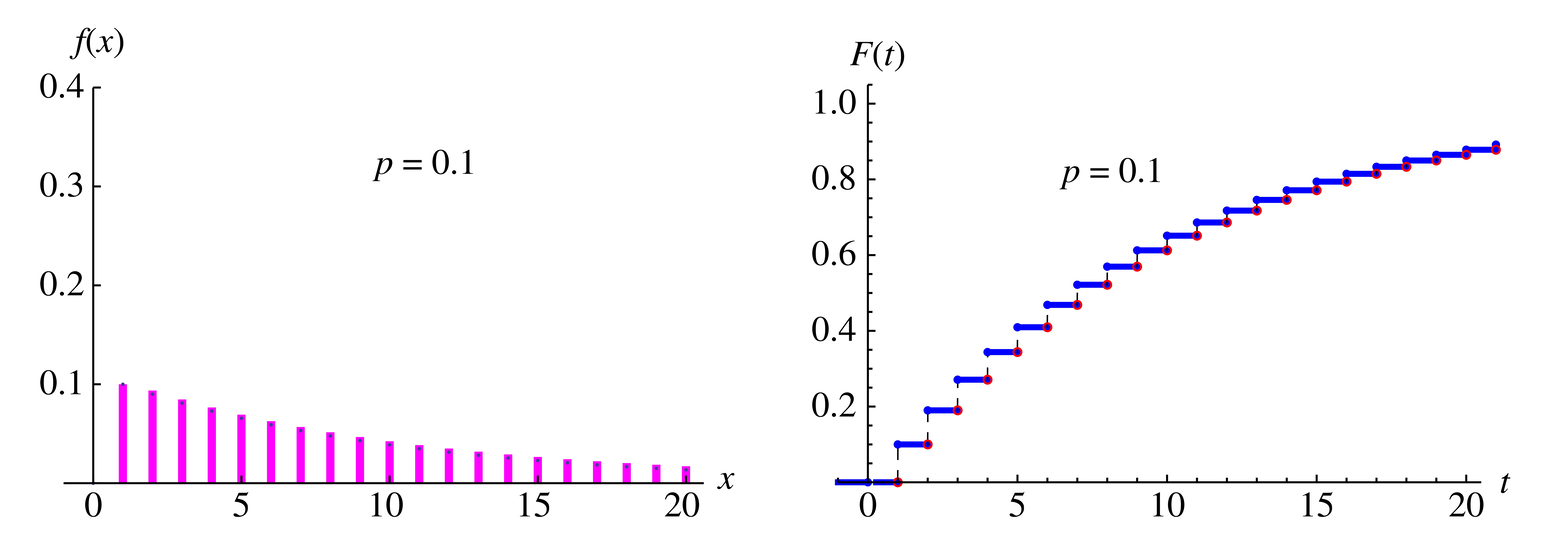
\includegraphics[width=1\linewidth]{geom.png}
Geométrica $G(p)$.
Número $n$ de ensayos de Bernoulli independientes con la misma probabilidad de éxito $p$, hasta obtener el primer éxito.
\begin{equation}\begin{matrix}
f(x)=q^{x-1},\\
x=1,2,\ldots,n;\\
E(X)=\frac{1}{p},\ Var(X)=\frac{q}{p^2}
\end{matrix}\end{equation}\end{subfigure}
\end{figure}


\begin{figure}[H]
\begin{subfigure}[t]{.475\textwidth}\includegraphics[width=1\linewidth]{negativabinominal.png}
Negativa binominal $Nb(rp)$. Número $n$ de ensayos de Bernoulli independientes con la misma probabilidad de éxito $p$, hasta obtener resultado número $r$.
\begin{equation}\begin{matrix}
f(x)=\binom{x-1}{r-1}p^rq^{x-r},\\
r=r,r+1,r+2,\ldots,n;\\
E(X)=\frac{r}{p},\ Var(X)=\frac{rq}{p^2}
\end{matrix}\end{equation}\end{subfigure}\qquad
\begin{subfigure}[t]{.475\textwidth}\includegraphics[width=1\linewidth]{hyperg.png}
Hipergeométrica $h(n;a,b)$. Muestra aleatoria tamaño $n$ de elementos tipo $a$ no reemplazada de un universo con elementos tipo $a$ y $b$.
\begin{equation}\begin{matrix}
f(x)=P(X=x)=\frac{\binom{a}{x}\binom{b}{n-x}}{\binom{a+b}{n}};\\
E(X)=n\cdot\frac{a}{a+b},\\
Var(X)=n\cdot\frac{a}{a+b}\cdot\frac{b}{a+b}\cdot(1-\frac{n-1}{a+b-1})
\end{matrix}\end{equation}\end{subfigure}
\end{figure}


\begin{figure}[H]
\begin{subfigure}[t]{.475\textwidth}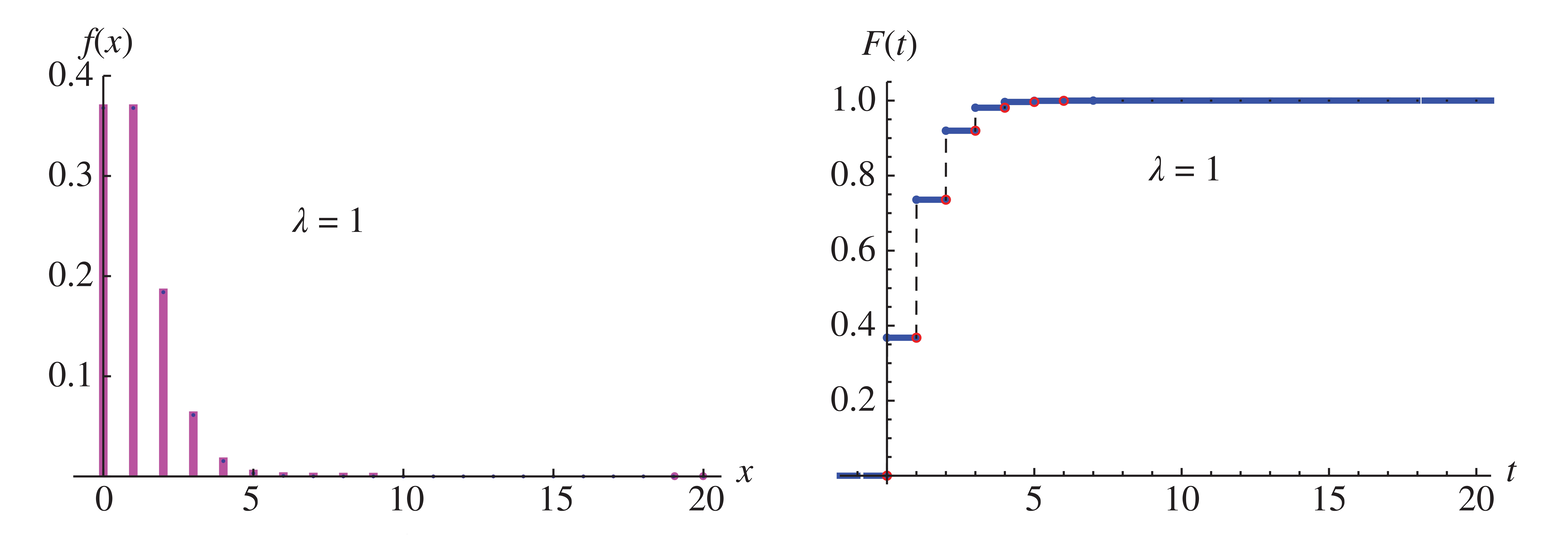
\includegraphics[width=1\linewidth]{poisson.png}
Poisson $\mathcal{P}(\lambda)$. Puede utilizarse con algún parámetro $\lambda$ cuando la probabilidad de éxito tiende a cero $(p\rightarrow0)$ de forma que la media $E(X)=np$ converge en algún $\lambda>0$.
\begin{equation}\begin{matrix}
f(x)=e^{-\lambda}\frac{\lambda^x}{x!},\\
x=0,1,2,\ldots;\\
E(X)=\lambda, Var(X)=\lambda
\end{matrix}\end{equation}\end{subfigure}\qquad
\begin{subfigure}[t]{.475\textwidth}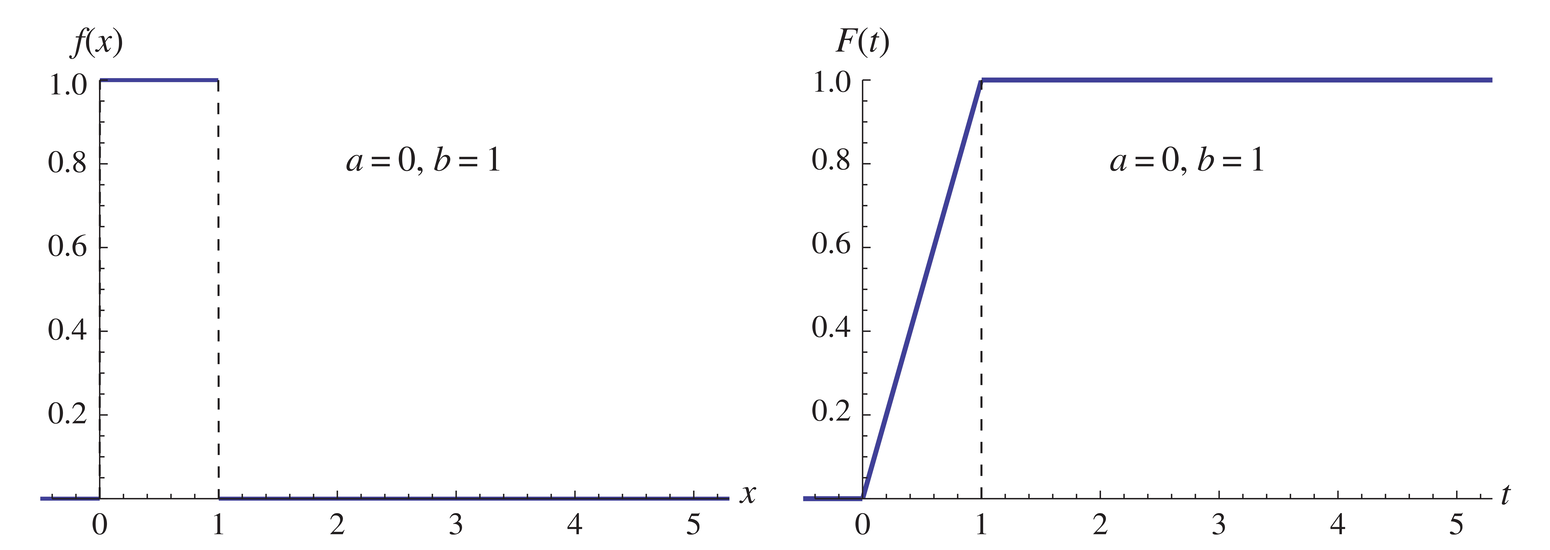
\includegraphics[width=1\linewidth]{uniforme.png}
Uniforme $U[a,b]$. Útil para modelar situaciones en que todos los intervalos tengan la misma amplitud y probabilidad.
\begin{equation}\begin{matrix}
f(x)\begin{cases}\frac{1}{b-a},\quad a\leq x\leq b,\\\text{de otro modo},\quad 0;\end{cases}\\
F(t)\begin{cases}0,\quad t<0,\\\frac{t-a}{b-a},\quad a\leq t\leq b,\\1,\quad t>b;\end{cases}\\
E(X)=\frac{a+b}{2},\quad Var(X)=\frac{{(b-a)}^2}{12}
\end{matrix}\end{equation}\end{subfigure}
\end{figure}


\begin{figure}[H]
\begin{subfigure}[t]{.475\textwidth}\includegraphics[width=1\linewidth]{normal.png}
Normal $N(\mu,\sigma^2)$. La suma y el promedio de un gran número de observaciones para una variable $X$ puede ser aproximada por la distribución normal, independientemente de su distribución original.
\begin{equation}\begin{matrix}
f(x)=\frac{1}{\sigma\sqrt{2\pi}}e^{-({x-\mu)}^2/(2\sigma^2)},\\
-\infty<z<\infty;\\
E(X)=\mu,\ Var(X)=\sigma^2
\end{matrix}\end{equation}\end{subfigure}\qquad
\begin{subfigure}[t]{.475\textwidth}\includegraphics[width=1\linewidth]{epsilon_lambda.png}
Exponencial $\epsilon(\lambda)$. Es considerada la análoga continua de la distribución geométrica y puede ser utilizada para modelar parte de la vida de un sujeto $X$.
\begin{equation}\begin{matrix}
f(x)=\begin{cases}\lambda^{-\lambda x},\ x\leq0,\\0,\ x<0;\end{cases}\\
F(t)=\begin{cases}0,\ t<0,\\1-e^{-\lambda t},\ x\geq 0;\end{cases}\\
E(X)=\frac{1}{\lambda},\ Var(X)=\frac{1}{\lambda^2}
\end{matrix}\end{equation}\end{subfigure}
\end{figure}

\begin{figure}[H]
\begin{subfigure}[t]{.475\textwidth}\includegraphics[width=1\linewidth]{gama.png}
Gama. Generalización de la distribución \emph{Erlang} cuando el parámetro $n$ no es necesariamente un entero.
\begin{equation}\begin{matrix}
f(x)=\begin{cases}\frac{\lambda^a}{\Gamma(a)}x^{a-1}e^{-\lambda x},\ x\geq 0,\\0,\ x<0,\end{cases}\\
\text{donde }\Gamma(a)=\int_{0}^{\infty}t^{a-1}e^{-t}dt\\\text{ es la función gama.}\\
E(X)=\frac{a}{\lambda},\ Var(X)=\frac{a}{\lambda^2}
\end{matrix}\end{equation}\end{subfigure}\qquad
\begin{subfigure}[t]{.475\textwidth}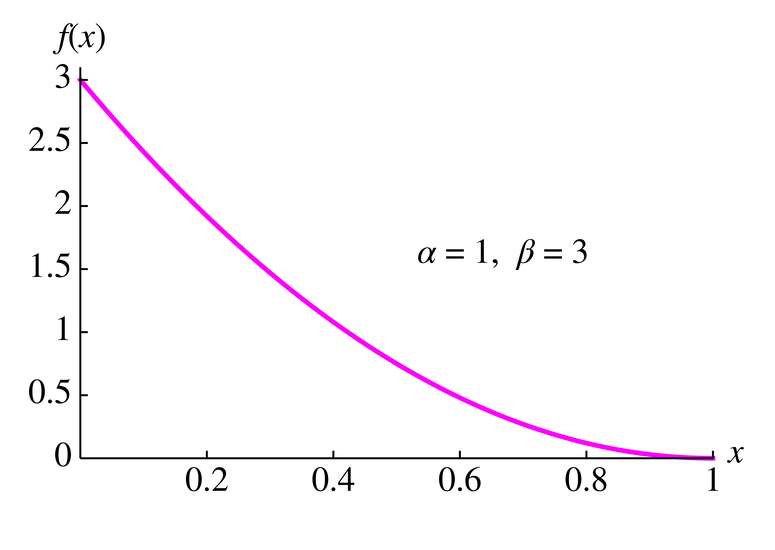
\includegraphics[width=1\linewidth]{beta.png}
Beta. Ofrece modelos satisfactorios para v.a.c.s que toman valores entre dos puntos conocidos.
\begin{equation}\begin{matrix}
f(x)=\begin{cases}\frac{1}{B(\alpha,\beta)}x^{\alpha-1}(1-x)^{\beta-1},\ 0<x<1,\\\text{de otro modo,}\ 0,\end{cases}\\
\text{donde } B(\alpha,\beta)=\\
\int_{0}^{1}x^{\alpha-1}(1-x)^{\beta-1}dx=\\
(\Gamma(\alpha)\Gamma(\beta)\big)/\big(\Gamma(\alpha+\beta)\big)\\
\text{es la función beta.}\\
E(X)=\frac{a}{\lambda},\ Var(X)=\frac{a}{\lambda^2}
\end{matrix}\end{equation}\end{subfigure}
\end{figure}